\chapter{Desenvolvimento do novo Portal \\FlossCoach}

Neste capítulo explicaremos como foi desenvolvido o novo portal FlossCoach, passando
pelas 3 fases passadas até o presente momento, desde a versão inicial até o FlossCoach
como está.

O desenvolvimento do novo Portal FlossCoach foi dividido em tres fases. Na primeira, 
nós construimos um protótipo funcional com base no FlossCoach atual. Nós coneçamos o
desenvolvimento do protótipo funcional pelos motivos citados na Seção~\ref{flosscoach},
que já não atendia mais as demandas que vinha recebendo.

O objetivo desta primeira fase do desenvolvimento era que obtivéssemos como cadastrar 
os projetos com os campos para cadastro que já eram relatados no portal \\FlossCoach 
além de do cadastro de usuários.

Para a obtenção desse cadastro, tivemos algumas conversas com o Igor para que chegássemos
a um modelo de dados inicial, onde contivesse todos os itens que já estavam presentes no
FlossCoach atual e os relacionamentos que ele gostaria que huvessem entre os elementos.

\begin{figure}[h]
	\centering
	\label{fig:diagrama_iicial}
		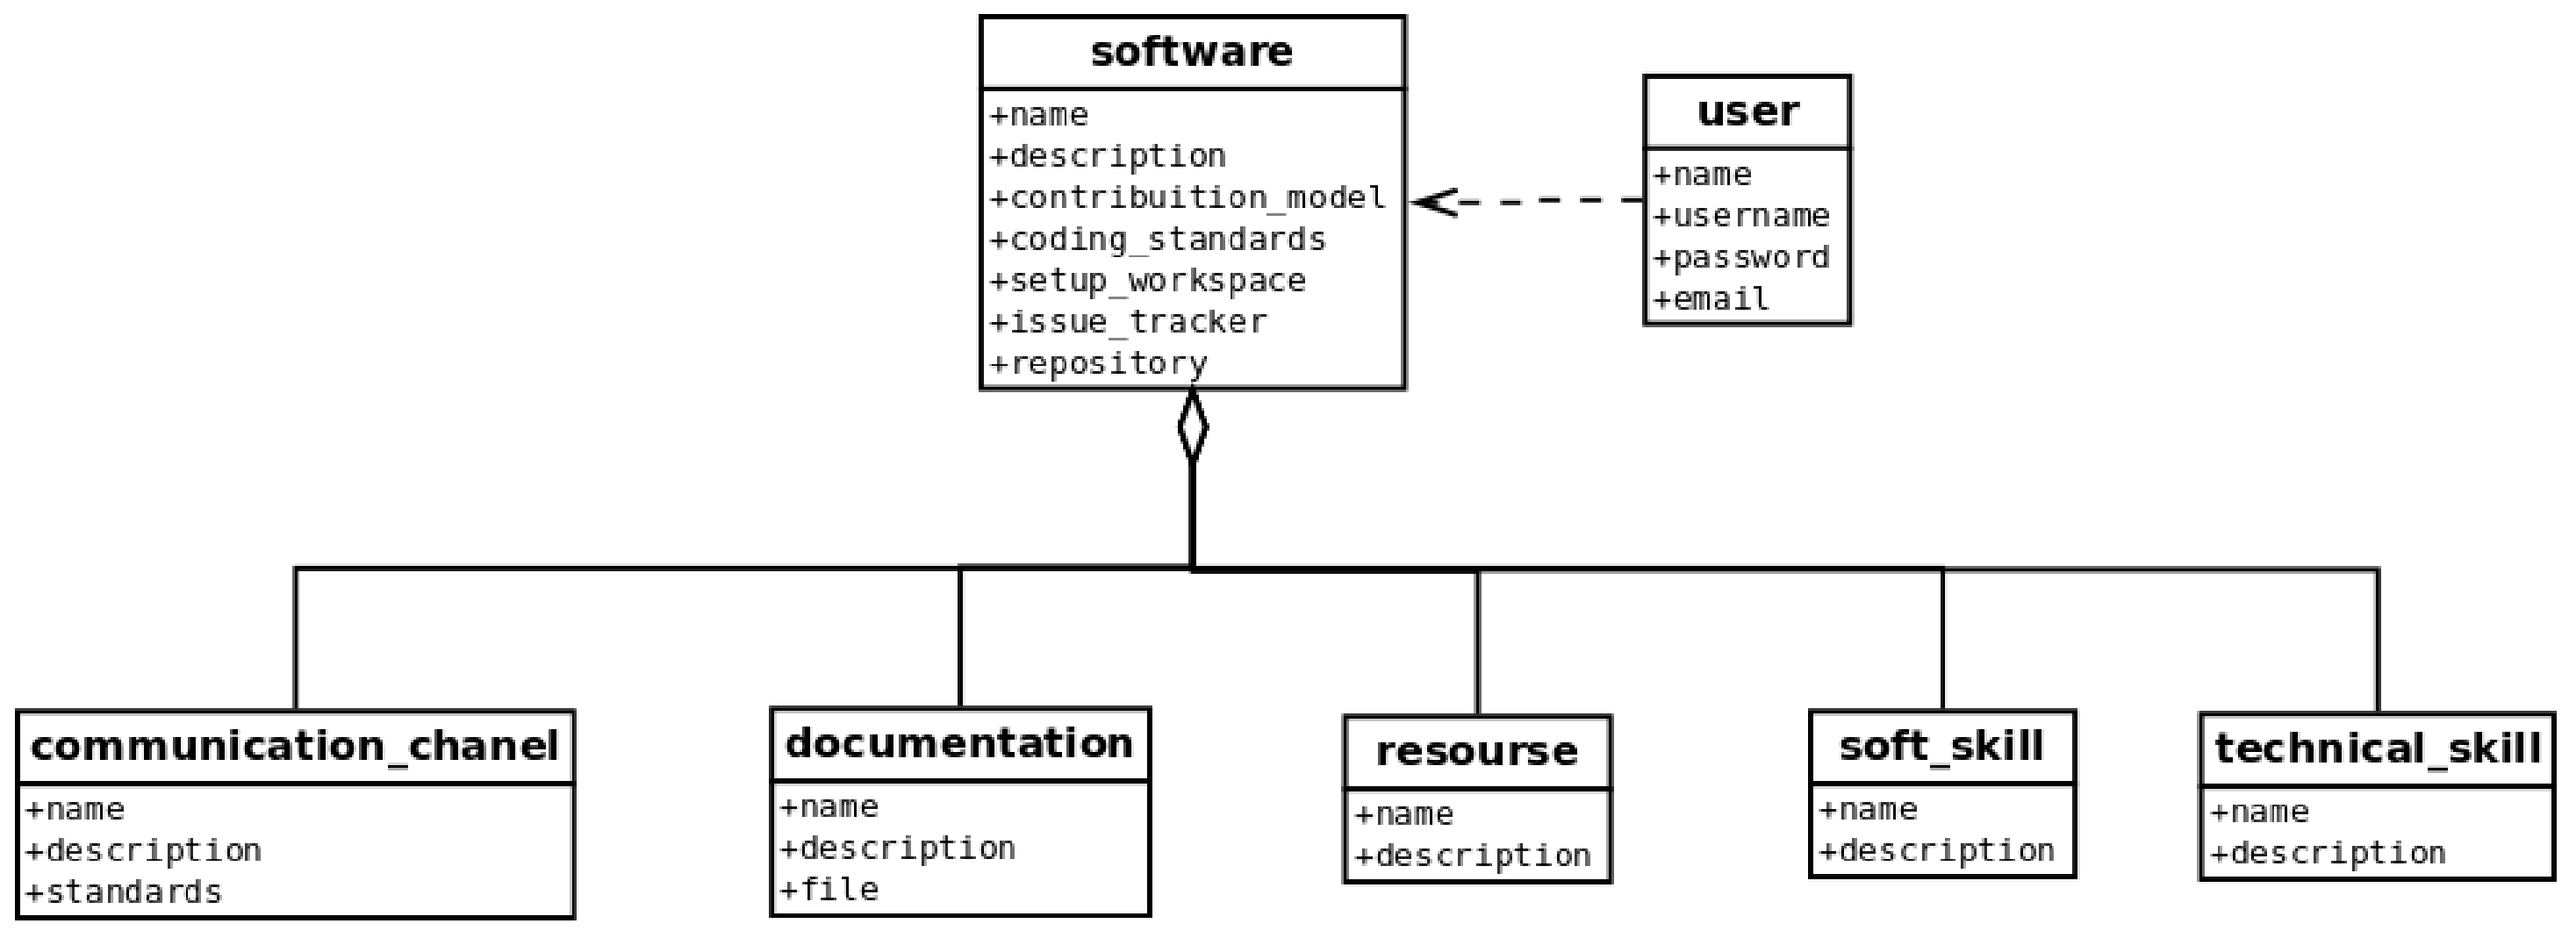
\includegraphics[keepaspectratio=true,scale=0.35]{figuras/diagrama_inicial.eps}
	\caption{Modelo de dados inicial do novo FlossCoach.}
\end{figure}

O protótipo funcional foi desenvolvido em \textit{ruby on rails} e \textit{bootstrap},
nós escolhemos estas tecnologias por serem amplamente utilizadas para desenvolvimento
de aplicações \textit{web} pela comunidade de software livre. Procuramos também utilizar
apenas de recursos de software livre para o desenvolvimento, incluindo a ferramenta de 
controle de versão e as bibliotecas utilizadas no \textit{front end}.

\begin{figure}[h]
	\centering
	\label{fig:prototipo}
		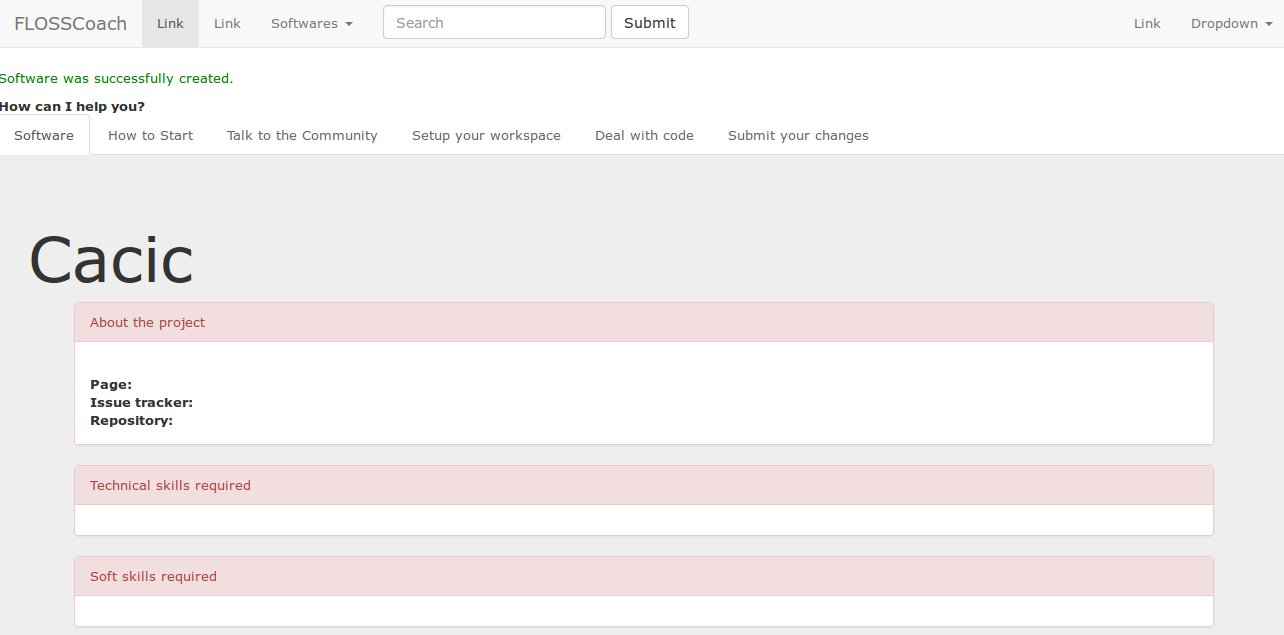
\includegraphics[keepaspectratio=true,scale=0.3]{figuras/prototipo.eps}
	\caption{Protótipo inicial do novo FlossCoach.}
\end{figure}

Esta fase do desenvolvimento durou 4 meses, iniciamos levantando os dados para implementação
em dezembro de 2015 e concluímos em março de 2016 quando nós passamos o código para o
professor Igor Steinmancher tomar conhecimento e iniciar a segunda fase do desenvolvimento.  


Na segunda fase do desenvolvimento o professor Igor Steinmancher montou uma equipe 
de desenvolvimento na USP, eles fizeram uma análise daquilo que nós havímos desenvolvido
e fizeram modificações no modelo de dados da aplicação chegando a uma segunda versão do 
modelo.

\begin{figure}[h]
	\centering
	\label{fig:diagrama_fase2}
		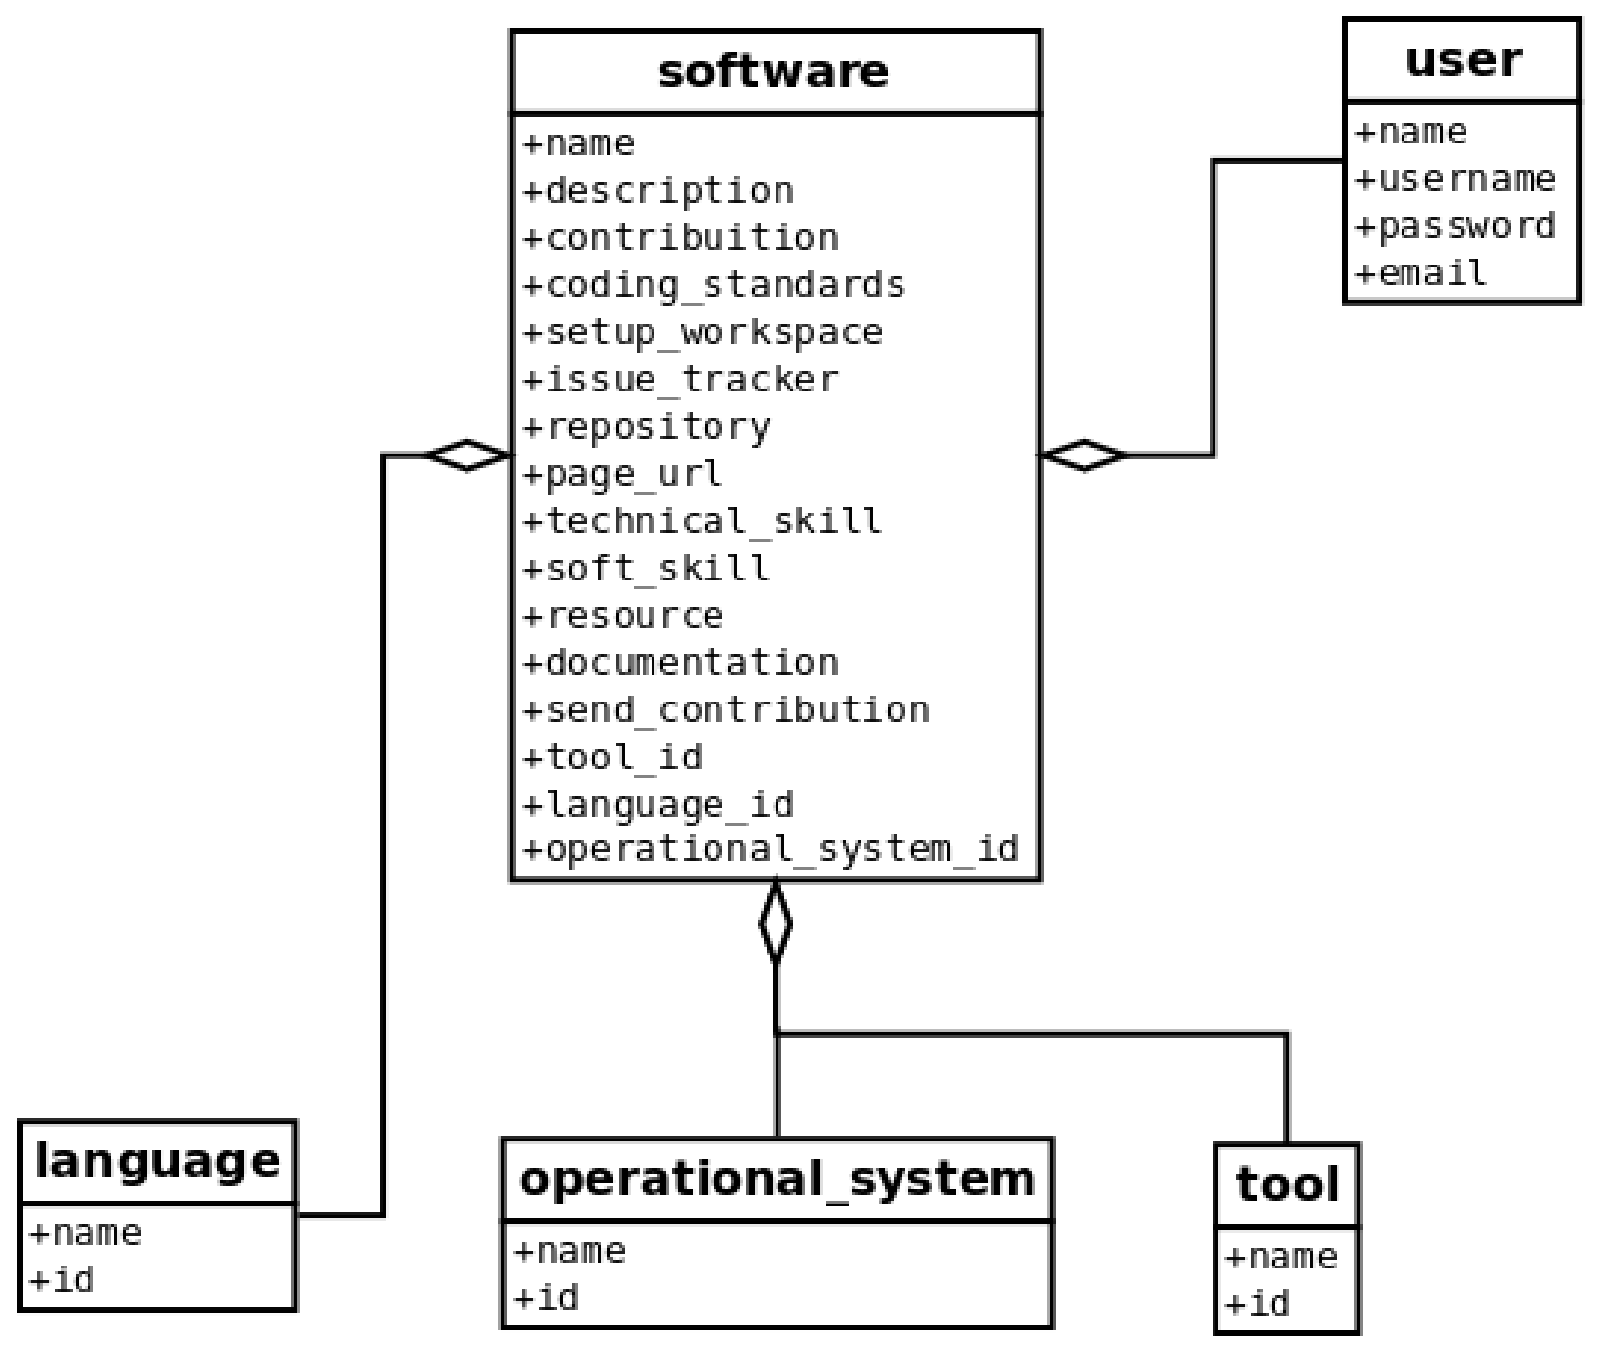
\includegraphics[keepaspectratio=true,scale=0.3]{figuras/diagrama_fase2.eps}
	\caption{Segunda versão do modelo de dados do novo FlossCoach.}
\end{figure}

Neste segunda versão no modelo de dados algumas classes deixaram de exixtir e se tornaram
atributos da classe \textit{software} e eles apresentaram 3 novas classes que não havia
no diagrama anterior. Eles implemetaram as modificações que fizeram no diagrama de dados
e melhoraram o \textit{front end} da aplicação além de desenvolver novas funcionalidades. 
Nesta etapa eles desenvolveram:
\begin{itemize}
\item Novo \textit{design} da aplicação;
\item Página de \textit{login}; 
\item \textit{Login} através de redes sociais;
\item Menu com barra lateral;
\item Modo tela cheia.
\item Consumo da API do \textit{Open hub}.
\end{itemize}

\begin{figure}[h]
	\centering
	\label{fig:prototipo}
		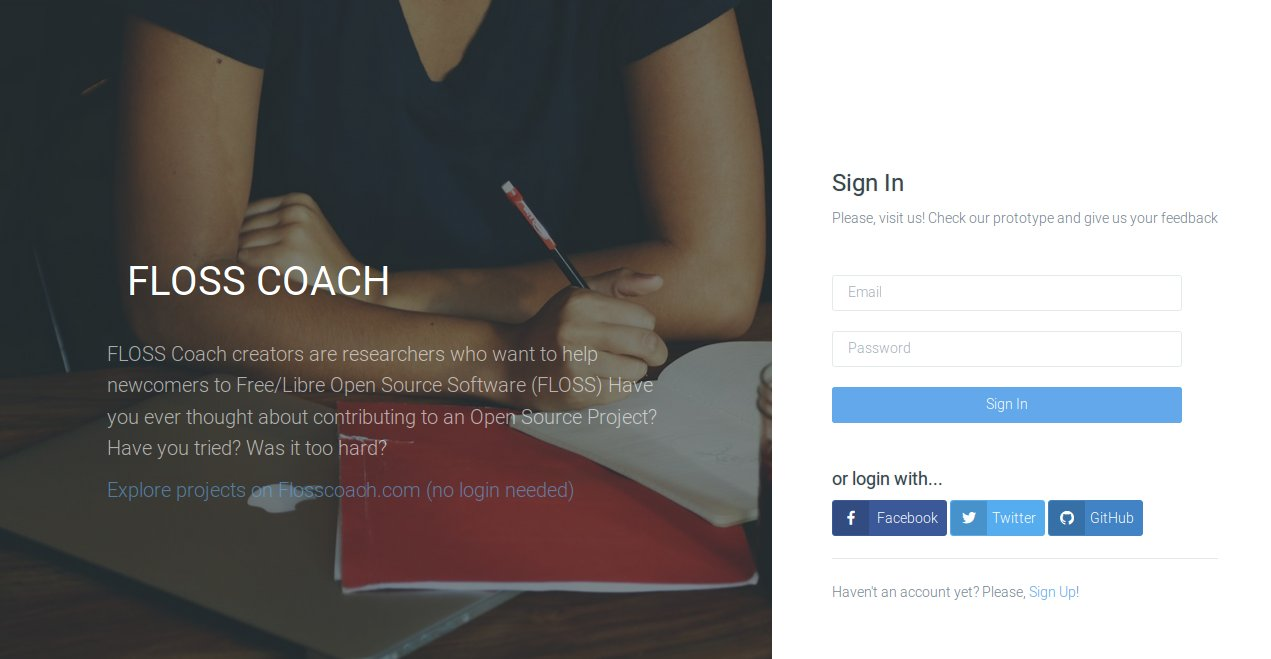
\includegraphics[keepaspectratio=true,scale=0.3]{figuras/login.eps}
	\caption{Página de \textit{login} inicial do novo FlossCoach.}
\end{figure}


\begin{figure}[h]
	\centering
	\label{fig:prototipo}
		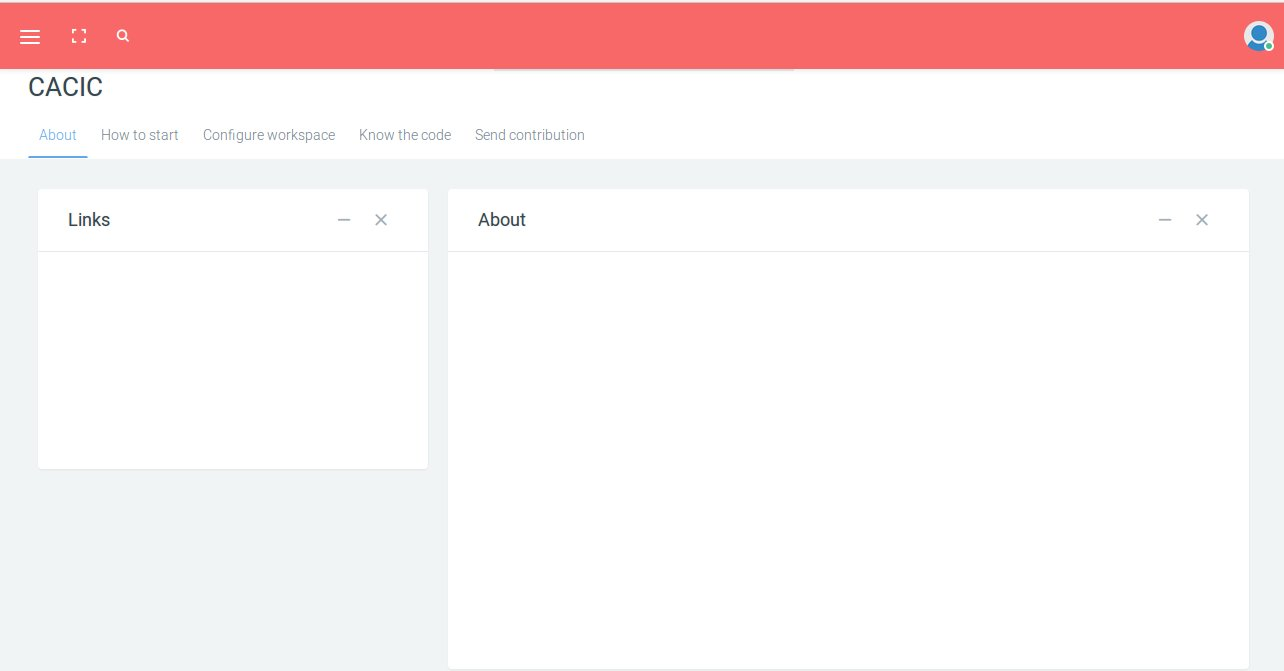
\includegraphics[keepaspectratio=true,scale=0.3]{figuras/layout.eps}
	\caption{\textit{Layout} do novo FlossCoach.}
\end{figure}


Neste intervalo de tempo da segunda fase nós traduzimos os questionários extraídos
da tese do professor Igor e adaptamos para o contexto de software público além de 
enviarmos os questionários para o grupo de interesse explicado no Capítulo~\ref{metodologia}.
Esta fase também durou 4 meses, tendo início em abril de 2016 e finalizando em julho de 2016.


%explcar terceira fase e sprints e todo o mecanismo da disciplina de mes

\begin{table}[h]
	\centering
	\label{tab01}
	
	\begin{tabular}{ccc}
		\toprule
		\textbf{Sprint} & \textbf{Issues desenvolvidas} \\
		\midrule
		Sprint 1 & Testes unitários das \textit{models} \\
			 & Levantar ambiente e tomar conhecimento do FlossCoach \\
		\midrule
		Sprint 2 & Criar papel de administrador do projeto\\
			 & Atribuir papel de administrador ao usuário que cria o projeto \\
			 & Aprovação de membros em projetos \\
		\midrule		
		Sprint 3 & Internacionalização \\
			 & \\
		\midrule		
		Sprint 4 & \\
		\midrule		
		Sprint 5 & \\
		\midrule
		Sprint 6 & \\
		\bottomrule
	\end{tabular}

	\caption{Conteúdo das sprints da terceira fase do desenvolvimento.}
\end{table}
